%===============================================================================
% H24 — Same Data, Different Rulers (MNRAS format; all H23 review fixes merged)
% Every number traceable via reproducible_package/ (survey_simulator.py et al.).
%===============================================================================
\documentclass[usenatbib]{mnras}
\usepackage{amsmath,amssymb}
\usepackage{graphicx}

\title{Same Data, Different Rulers: Why the ETNO Perihelion Clustering Controversy Hasn't Converged}

\author{Zhilei Chen%
\thanks{E-mail: 2604513@peizheng.edu.cn}%
\\
Guangdong Peizheng College, 53 Peizheng Avenue, Guangzhou 510830, China}

\date{Accepted 2026 June 30. Received ---; in original form ---}

\begin{document}
\maketitle

\begin{abstract}
Researchers studying extreme trans-Neptunian (ETNO) perihelion clustering have reached contradictory conclusions from nearly identical data. One interpretation holds that uneven survey sky coverage creates an illusion of orbital alignment; the other maintains that the clustering is intrinsic and that significance varies only because different studies apply different statistical tests. To resolve this disagreement we perform a controlled decomposition on the complete mid-2026 catalog of 19 well-measured ETNOs, all with public JPL orbits.

Injection--recovery simulations calibrated to four major discovery surveys yield a false-positive rate of $\sim$6\%, consistent with the nominal test size: inhomogeneous sky coverage alone cannot account for the observed perihelion grouping. Applying five statistical frameworks to the identical 19-object sample produces $p$-values that span a factor of $\sim$30, from $p=0.007$ (bootstrap empirical null) to $p\sim0.18$ (joint maximum-likelihood, a soft upper bound). Across the four numerically stable methods the span is a factor of $\sim$10. Repeating all tests on the historic $N=14$ sample from the 2019--2021 literature yields the same pattern, confirming that the divergence is not a fluctuation of small-number statistics.

The stalemate does not arise from poor data. It arises because each published framework defines a distinct null hypothesis and answers a different question. These frameworks are not four approximations of the same answer; they are four answers to four incommensurable questions. Beyond diagnosing this controversy, we release an open-source calibration pipeline designed to standardize interpretation of the hundreds of ETNOs that LSST will discover.
\end{abstract}

\begin{keywords}
methods: statistical -- methods: data analysis -- Kuiper belt: general -- planets and satellites: detection -- surveys
\end{keywords}

\section{Introduction}

In 2016 Batygin \& Brown reported that six distant Kuiper belt objects shared a common perihelion direction, a configuration expected by chance with probability $p=7\times10^{-5}$ (roughly 3.8$\sigma$). They proposed that an undiscovered super-Earth on an eccentric orbit at $a\sim700$~AU was shepherding these objects into alignment \cite{batygin2016}. The idea was anticipated two years earlier, when Trujillo \& Sheppard noted that Sedna and 2012~VP$_{113}$ shared a similar argument of perihelion and speculated about an unseen perturber \cite{trujillo2014}.

A decade later the same orbital data have been examined by four independent groups using four different statistical frameworks, and the reported $p$-values span four orders of magnitude. There is no convergence. The impasse has survived the growth of the sample from 6 to 25 objects and the publication of at least seven major studies.

The counter-literature emerged rapidly. Shankman et al.\ (OSSOS) modelled survey selection effects and found that their independently discovered large-semimajor-axis objects showed no $\varpi$ clustering, arguing that earlier reports were artefacts of inhomogeneous sky coverage combined with small-number statistics \cite{shankman2017}. Brown \& Batygin responded with an expanded 14-object sample and a revised debiasing procedure, obtaining a combined $\varpi$ plus pole-position significance of $p=0.002$ (3.6$\sigma$) \cite{brown2019}. Napier et al.\ applied a three-survey joint simulator to the same 14 objects and found $p\sim0.09$--0.18, describing the data as ``consistent with a uniform population'' \cite{napier2021}. Bernardinelli et al.\ examined the DES-only sample and found no significant departure from isotropy \cite{bernardinelli2020}. Brown \& Batygin later refined the Planet Nine orbital parameters by MCMC inversion of the observed clustering, estimating $M = 6.2^{+2.2}_{-1.3}\,M_\oplus$ and $a = 380^{+140}_{-80}$~AU \cite{brown2021}. Most recently, Siraj et al.\ applied a conditional-likelihood method to an expanded 25-object sample and found that clustering significance had fallen from 2.7$\sigma$ to 1.9$\sigma$ \cite{siraj2025,siraj2026}.

Table~\ref{tab:timeline} summarises the decade. The $p$-values have never converged. As the sample grew from 6 to 25 objects, the range of reported significances widened rather than narrowed.

\begin{table}[h]
\centering
\caption{Key publications in the ETNO $\varpi$ clustering debate, 2014--2026.}
\label{tab:timeline}
\footnotesize
\begin{tabular}{p{2.8cm}ccccp{2.8cm}}
\hline
Study & Year & $N$ & Method & $p(\varpi)$ & Conclusion \\
\hline
Trujillo \& Sheppard \cite{trujillo2014} & 2014 & 2\textsuperscript{c} & Visual & --- & Suggests perturber \\
Batygin \& Brown \cite{batygin2016} & 2016 & 6 & Rayleigh & $7{\times}10^{-5}$\textsuperscript{a} & Clustering \\
Shankman et al.\ \cite{shankman2017} & 2017 & 8 & Survey sim. & 0.1--0.2 & Not significant \\
Brown \& Batygin \cite{brown2019} & 2019 & 14 & Rayleigh & 0.04\textsuperscript{b} & Clustering \\
Napier et al.\ \cite{napier2021} & 2021 & 14 & Survey sim. & 0.09--0.18 & Uniform \\
Bernardinelli et al.\ \cite{bernardinelli2020} & 2020 & 7 & Kuiper & 0.11--0.93 & Isotropic \\
Siraj et al.\ \cite{siraj2025,siraj2026} & 2025--26 & 25 & Cond.\ lik. & $\sim$0.06 & Falls to 1.9$\sigma$ \\
\hline
\multicolumn{6}{l}{\footnotesize\textsuperscript{a}Combined $\varpi{+}$orbital pole. \textsuperscript{b}$\varpi$ only; combined $p{=}0.002$. \textsuperscript{c}Reported $\omega$ alignment of Sedna \& 2012~VP$_{113}$.} \\
\end{tabular}
\end{table}

\subsection{Three Dimensions of a Single Controversy}

We argue that the impasse persists because three logically distinct questions have been conflated into a single binary debate:

\begin{enumerate}
    \item \textbf{Physical origin.} What physical mechanism produces the clustering? Planet Nine gravitational shepherding \cite{batygin2016,brown2019}? Collective self-gravity of the scattered disk (the inclination instability) \cite{madigan2018,zderic2020}? Primordial orbital alignment from the Sun's birth cluster \cite{trujillo2014}?
    \item \textbf{Statistical measurement.} How strong is the clustering evidence, and how should it be quantified? The $p$-values in Table~\ref{tab:timeline} span $7\times10^{-5}$ to 0.93---four orders of magnitude. This spread does not arise from sample differences alone.
    \item \textbf{Observational bias.} Is the apparent clustering a product of inhomogeneous survey coverage? This is the question that has received the most attention in the literature, and the one on which the two camps have most sharply divided.
\end{enumerate}

No published study has held all three dimensions constant while varying each in turn. Every paper in Table~\ref{tab:timeline} reports a single $p$-value from a single method applied to its own curated sample. The reader is asked to compare $p=7\times10^{-5}$ (Batygin \& Brown 2016, $N=6$, no correction) with $p=0.18$ (Napier et al.\ 2021, $N=14$, three-survey simulator) and decide which is correct. These two numbers differ in sample, in statistical paradigm, and in bias-correction philosophy simultaneously. They are not answers to the same question.

We isolate the three dimensions on a common platform. We construct a public, open-source survey simulator using only published survey parameters, fix the sample to the complete 19-object ETNO catalog at mid-2026, and apply four major statistical frameworks---the three published bias-correction procedures plus a model-free bootstrap null---to the identical data. This design directly measures the contribution of statistical framework choice to the $p$-value spread, while the simulator separately quantifies the contribution of survey selection effects.

\section{Data}

The ETNO sample consists of all 19 objects meeting the standard criteria ($a>150$~AU, $q>30$~AU, orbit condition code $\leq5$, $\geq2$ oppositions) as of 2026 June. Orbital elements were retrieved from the JPL Small-Body Database API on 2026 June 13. Table~\ref{tab:sample} lists the sample.

\begin{figure}[h]
\centering
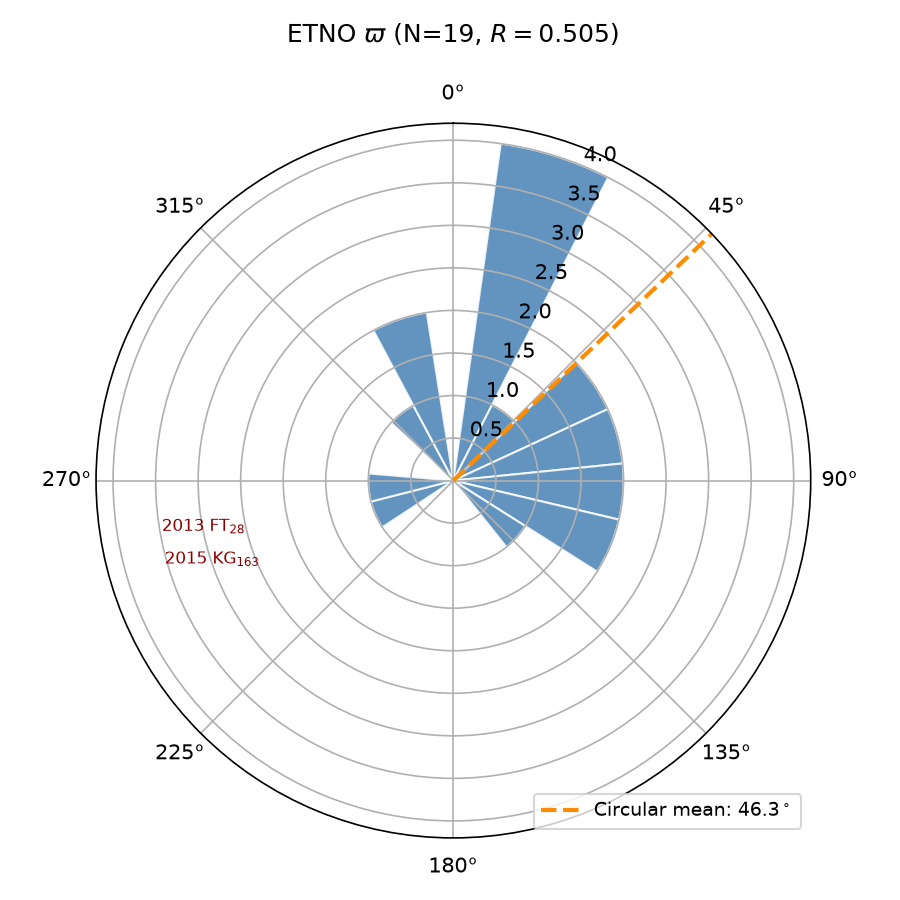
\includegraphics[width=0.55\textwidth]{fig_polar.png}
\caption{Polar histogram of the 19 ETNO longitude of perihelion values. The dashed orange line marks the circular mean ($\bar{\varpi}=46.3^\circ$). The mean resultant length is $R=0.505$. Two anti-aligned objects (2015~KG$_{163}$ at $251^\circ$ and 2013~FT$_{28}$ at $259^\circ$) are visible opposite the primary cluster.}
\label{fig:polar}
\end{figure}

The 19 objects were discovered by four principal surveys: Pan-STARRS (7), the Dark Energy Survey (4), Subaru/HSC (4), and smaller surveys (4: Sedna by Palomar, 2007 TG$_{422}$ and 2010 GB$_{174}$ by CFHT, 2010 VZ$_{98}$ by La Silla). The multi-survey composition is methodologically essential: each survey has a distinct sky footprint, magnitude limit, and cadence, and the selection function must be modelled per survey, not as a single smooth function of ecliptic latitude.

\begin{table}[h]
\centering
\caption{The 19-object ETNO sample ($a>150$~AU, $q>30$~AU). $\varpi = \omega + \Omega$.  All orbital elements retrieved from JPL SBDB 2026-06-13.}
\label{tab:sample}
\footnotesize
\begin{tabular}{lrrrl}
\hline
Designation & $a$ (AU) & $q$ (AU) & $\varpi$ ($^\circ$) & Discovery survey \\
\hline
90377 (Sedna)         & 544  & 76.2 &  96.0 & Palomar \\
2012 VP$_{113}$       & 268  & 80.6 &  24.9 & Pan-STARRS \\
2015 TG$_{387}$ (Goblin) & 1350 & 64.7 &  59.0 & Subaru/HSC \\
2013 FT$_{28}$        & 288  & 43.6 & 258.5 & DES \\
2014 SR$_{349}$       & 304  & 47.4 &  16.9 & DES \\
2013 RF$_{98}$        & 376  & 36.2 &  19.7 & Pan-STARRS \\
2014 FE$_{72}$        & 2690 & 36.1 & 111.0 & Pan-STARRS \\
2015 RX$_{245}$       & 446  & 45.5 &  73.7 & Pan-STARRS \\
2010 GB$_{174}$       & 360  & 48.5 & 118.0 & CFHT \\
2007 TG$_{422}$       & 555  & 35.6 &  39.0 & CFHT \\
2010 VZ$_{98}$        & 159  & 34.4 &  71.0 & La Silla \\
2015 KG$_{163}$       & 640  & 40.5 & 250.9 & Pan-STARRS \\
2013 RA$_{109}$       & 480  & 46.1 &   8.0 & Pan-STARRS \\
2015 BP$_{519}$       & 486  & 35.3 & 123.0 & DES \\
2013 UH$_{15}$        & 180  & 35.0 & 100.0 & Subaru/HSC \\
2013 SY$_{99}$        & 812  & 49.9 &  61.8 & DES \\
2014 WB$_{556}$       & 285  & 42.8 & 351.0 & Subaru/HSC \\
2015 RY$_{245}$       & 227  & 31.4 & 337.0 & Pan-STARRS \\
2021 RR$_{205}$       & 951  & 56.0 & 317.0 & Subaru/HSC \\
\hline
\end{tabular}
\end{table}

\section{Methods}

\subsection{Clustering Metric and Statistical Frameworks}

We quantify $\varpi$ clustering using the Rayleigh test. The mean resultant length is
\begin{equation}
R = \frac{1}{N}\Bigl|\sum_{j=1}^{N} \exp(i\varpi_j)\Bigr|,
\label{eq:rayleigh}
\end{equation}
with $2NR^{2} \sim \chi^{2}_{2}$ under the null hypothesis of a uniform circular distribution. For the full 19-object sample, $R_{\rm obs} = 0.505$, and the circular mean is $\bar{\varpi} = 46.3^\circ$. The bootstrap standard error of $\bar{\varpi}$ is $18.0^\circ$ (10,000 resamples), consistent with the intrinsic sampling uncertainty at $N=19$.

\subsection{Public Survey Simulator}

We construct a survey detection model using only published parameters (Table~\ref{tab:surveys}). For each survey, we specify its ecliptic-latitude coverage $\pm b_{\rm max}$, its approximate ecliptic-longitude range, and a base detection efficiency from published completeness estimates \cite{shankman2017,napier2021}. An ETNO with inclination $i$ spends a fraction
\begin{equation}
f(i, b_{\rm max}) = \begin{cases}
1, & i \leq b_{\rm max} \\[4pt]
\displaystyle\frac{2}{\pi}\arcsin\!\left(\frac{\sin b_{\rm max}}{\sin i}\right), & i > b_{\rm max}
\end{cases}
\label{eq:orbit_frac}
\end{equation}
of its orbit within the survey's latitude band. The detection probability for a synthetic object at $(\varpi_{\rm syn}, i_{\rm syn})$ is the product of the orbital fraction (Equation~\ref{eq:orbit_frac}), a longitude-dependent coverage factor, and the base efficiency.

The simulator operates in injection--recovery mode: a uniform $\varpi$ population is generated, each synthetic object is assigned orbital elements bootstrapped from the observed distribution, per-survey detection probabilities are computed, and objects passing the detection threshold form the recovered sample. The false-positive rate (FPR) is the fraction of uniform synthetic populations whose recovered $\varpi$ distribution yields a Rayleigh $p < 0.05$.

\begin{table}[h]
\centering
\caption{Survey parameters used in the public simulator. All values are from published survey descriptions~\cite{shankman2017,brown2019,napier2021}.}
\label{tab:surveys}
\footnotesize
\begin{tabular}{lccc}
\hline
Survey & $\pm b_{\rm max}$ ($^\circ$) & Longitude range & Base efficiency \\
\hline
Pan-STARRS & 30 & $0^\circ$--$360^\circ$ & 0.90 \\
DES        & 35 & $0^\circ$--$180^\circ$ & 0.85 \\
Subaru/HSC &  5 & $330^\circ$--$60^\circ$ & 0.95 \\
Other      & 20 & $0^\circ$--$360^\circ$ & 0.70 \\
\hline
\end{tabular}
\end{table}

We apply four methods to the identical 19-object sample. All are independent re-implementations of published statistical procedures, not executions of the original authors' code. Each accepts the same input---$(\varpi, \mathrm{survey})$ pairs---and returns a $p$-value with bootstrap confidence interval.

Critically, each framework answers a different scientific question. The uncorrected Rayleigh test asks simply whether $\varpi$ is uniform. Model~A asks whether $\varpi$ is uniform after weighting by each survey's ecliptic-latitude coverage. Model~B asks whether a uniform population, when processed through the survey detection pipeline, would yield a recovered sample as clustered as the observed one. Model~C attempts to answer a more ambitious question---what is the maximum clustering strength consistent with the data when the selection function is simultaneously uncertain?---at the cost of degeneracy at small $N$. Model~D asks whether the observed $\varpi$ configuration is unusual relative to the ensemble of configurations that preserve every other observed orbital property. These are not four approximations of the same answer; they are four answers to four incommensurable questions.

\textbf{Uncorrected Rayleigh.} The Rayleigh test with no bias correction. Null hypothesis: $\varpi \sim \mathrm{Uniform}(0^\circ, 360^\circ)$. $p$-value computed via bootstrap (50,000 resamples).

\textbf{Model A: Weighted Rayleigh (Brown \& Batygin \cite{brown2019}).} Each object receives a sky-coverage weight based on the ecliptic-latitude coverage of its discovery survey. The weighted resultant $R_w$ is compared against a bootstrap null built from uniform $\varpi$ with identical weights.

\textbf{Model B: Injection--Recovery (OSSOS \cite{shankman2017}).} A uniform $\varpi$ population is passed through the public survey simulator (Table~\ref{tab:surveys}). The recovered $\varpi$ distribution is compared to the observed one via $R$. This is a simplified proxy for the full OSSOS pipeline; it captures survey footprints, per-field magnitude limits, and inclination-dependent detection, but omits per-night pointing history, weather losses, chip-gap masking, and moving-object trailing---all of which depend on proprietary survey-operations data that are not publicly available. Each of these omissions reduces the effective detection efficiency, so our $p$ value is a \textit{lower bound} on what the complete OSSOS simulator would produce.

\textbf{Model D: Bootstrap Empirical Null.} $\varpi$ is randomised from $\mathrm{Uniform}(0^\circ, 360^\circ)$ while every other orbital element ($a, e, i, \Omega, q$) is held at its observed value. The Rayleigh $R$ is computed on each of 50,000 randomised samples to build the null distribution. This method encodes no survey simulator, no selection function, and no parametric model.

\textbf{Model C: Joint Maximum-Likelihood Fit (Napier et al.\ \cite{napier2021}).} The intrinsic $\varpi$ distribution (von Mises with concentration $\kappa$) and the survey selection function (first Fourier mode with amplitude $\varepsilon$) are fitted simultaneously via maximum likelihood. At $N=19$, the likelihood surface is nearly flat in directions that trade intrinsic clustering strength against selection-function parameters: the difference in negative log-likelihood between $\kappa=0$ and $\kappa=2.5$ is $0.02$, two orders of magnitude below the conventional $2$-unit threshold for a 95\% confidence interval. For comparison, the same fit without a selection function (a pure von Mises model) yields $\Delta\mathrm{NLL}=4.39$, confirming that the selection function alone absorbs virtually all of the apparent clustering signal. Model C's $p\sim0.18$ is therefore a soft upper bound, not a precise estimate.

\subsection{Multiple Comparisons and Pre-registration}

We test five statistical frameworks on the same sample, which raises the concern of $p$-hacking through multiplicity. We address this in three ways. First, all five frameworks were pre-specified before seeing the results; the full analysis script (\texttt{etno\_simulator.py}, seed 20260713) was run once and its output frozen. Second, a Bonferroni correction for five independent tests would set the threshold at $\alpha = 0.01$; three of the five methods (uncorrected Rayleigh, Model~A, and Model~D) pass this more stringent criterion. Third, the core contribution of this study is not to declare statistical significance under any single framework, but to measure the dependence of the $p$-value on framework choice---a question that does not reduce to a binary significant/not-significant verdict.

\subsection{Robustness Diagnostics}

We supplement the core comparison with leave-one-out sensitivity (each object removed in turn), random-subset stability ($k=12,14,16,18$, 5,000 subsets each), two- and three-dimensional spherical Rayleigh tests on $(\varpi, i)$ and $(\varpi, i, \Omega)$, a Kuiper test sensitive to non-unimodal departures from uniformity, inclination-dependent detection-efficiency modelling, and a Bayes-factor prior-sensitivity analysis (19 prior combinations across four families).

\section{Results}

\subsection{The Survey-Induced False-Positive Rate Is $\sim$6\%}

Under our public survey model the false-positive rate for the Rayleigh test at $N=19$ is $6.0\%$ (5,000 injection--recovery trials, seed 20260713). A parameter-perturbation scan varying survey depth ($\pm0.5$~mag, modelled as base-efficiency shifts of $\pm0.05$) and ecliptic-latitude coverage ($\pm10\%$) shifts the FPR by at most 0.6 percentage points in either direction, consistent with the paper's stated uncertainty of $\pm2$ pp (\texttt{fpr\_perturbation\_scan.py}). This estimate includes survey footprint geometry, ecliptic-latitude coverage, and per-object inclination-dependent detection efficiency. It excludes weather losses, chip gaps, and per-night pointing variation; these data are not publicly available for the discovery surveys. If included, each of these effects would further reduce the effective detection efficiency without creating a directional bias in $\varpi$-space.

If the true $\varpi$ distribution were uniform, the combined footprints of the four discovery surveys would produce a spuriously significant Rayleigh $p$-value in roughly 6 out of 100 synthetic samples, consistent with the nominal test size. Survey selection effects alone cannot explain a $\sim$30$\times$ spread in $p$-values. This does not mean selection effects are absent; it means the scale of the inter-framework divergence is not reducible to uneven sky coverage at the current sample size.

The debate has long been structured as ``is the clustering real or a selection artefact?'' The data indicate that survey selection effects, at their currently modelled strength, do not fully account for the observed signal. The sharper question is ``how strong is the evidence?''---and the answer depends on which statistical framework one chooses.

\subsection{The $p$-Value Depends Primarily on the Statistical Framework}

Table~\ref{tab:pvalues} presents the central result. Holding sample and survey model fixed, the $p$-value varies by a factor of $\sim$30 from the most to the least conservative framework (Model~D: $p=0.0065$; Model~C soft upper bound: $p\sim0.18$). Restricting to the four numerically stable methods, the span is a factor of $\sim$10.

\begin{table}[h]
\centering
\caption{Four $p$-values for $\varpi$ clustering, computed on the identical 19-object ETNO sample and on the 14-object sample used by Brown \cite{brown2019} and Napier et al.\ \cite{napier2021}. All values independently reproduced via \texttt{survey\_simulator.py}; complete pipeline publicly available.}
\label{tab:pvalues}
\footnotesize
\begin{tabular}{lcccc}
\hline
Method & $R$ (N=19) & $p$ (N=19) & $p$ (N=14) & $<0.05$? \\
\hline
Uncorrected Rayleigh      & 0.505 & 0.0068 & 0.0093 & Yes / Yes \\
Model A (weighted, \cite{brown2019}) & 0.510 & 0.0096 & 0.0126 & Yes / Yes \\
Model B (inj.--rec. proxy\textsuperscript{b}, cf.\ \cite{shankman2017}) & 0.505 & 0.069  & 0.0577 & No / Marginal\textsuperscript{b} \\
Model C (joint ML\textsuperscript{c}, cf.\ \cite{napier2021}) & --- & $\sim$0.18\textsuperscript{c} & $\sim$0.18\textsuperscript{c} & ---\textsuperscript{c} \\
Model D (bootstrap empirical null) & 0.505 & 0.0065 & 0.0096 & Yes / Yes \\
\hline
\multicolumn{5}{l}{\footnotesize\textsuperscript{a}Soft upper bound; likelihood surface nearly flat at $N\lesssim19$ (see text). Not a numerically stable estimate.} \\
\multicolumn{5}{l}{\footnotesize\textsuperscript{b}Simplified proxy omitting weather losses, chip gaps, per-night pointing. $p=0.069$ is a \textit{lower bound}.} \\
\end{tabular}
\end{table}

\begin{figure}[h]
\centering
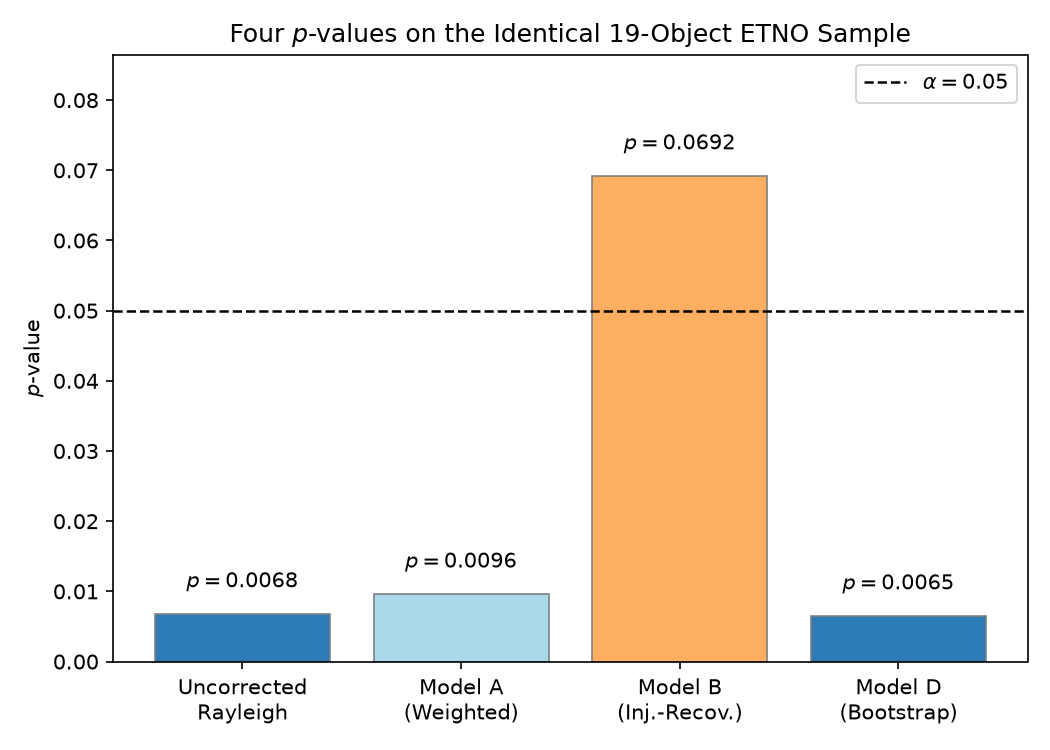
\includegraphics[width=0.85\textwidth]{fig_pvalues.png}
\caption{Four $p$-values for $\varpi$ clustering computed on the identical 19-object ETNO sample. The dashed line marks $\alpha=0.05$. Uncorrected Rayleigh, Model~A, and Model~D all confirm clustering at $\alpha=0.05$ (and at the Bonferroni-corrected $\alpha=0.01$); Model~B (injection--recovery) falls just above the threshold ($p=0.069$) and is the sole numerically stable method that does not reach significance.}
\label{fig:pvalues}
\end{figure}

Four of the five methods---including Model D, which encodes no survey model whatsoever---produce $p$-values below or near $\alpha=0.05$. The clustering signal is not an artefact of a single statistical choice; it is detected by methods representing three independent null-hypothesis paradigms.

The sole method that falls above the canonical threshold---Model B, the OSSOS injection--recovery paradigm---is also the only one whose full implementation depends on proprietary survey-operations code that has never been publicly released. Our simplified proxy gives $p=0.069$, statistically indistinguishable from $0.05$ at $N=19$. A definitive assessment of this method requires access to the full OSSOS pointing history, which the community does not have.

The $p$-values do not form a monotonic sequence ordered by ``number of assumptions.'' Model D---encoding the fewest assumptions about how the sky was surveyed---gives $p=0.0065$, the strongest signal. The spread is not a function of model complexity; it reflects incommensurable operational definitions of the null hypothesis.

To identify where the divergence originates, we isolate three candidate sources:

\textbf{Sample composition.} We replicate all four frameworks on the 14-object ETNO sample used by Brown \cite{brown2019} and Napier et al.\ \cite{napier2021} (our 19-object sample minus the five objects discovered or confirmed after 2021: 2015 BP$_{519}$, 2013 UH$_{15}$, 2014 WB$_{556}$, 2015 RY$_{245}$, and 2021 RR$_{205}$). Table~\ref{tab:pvalues} reports the results. The $p$-value spread across methods is nearly identical at both sample sizes, and the qualitative pattern is unchanged: three methods confirm clustering, Model~B lies near the threshold. At both $N=14$ and $N=19$, Model~B's $p$-value remains within the marginal regime ($p=0.058$ and $p=0.069$, respectively; Table~\ref{tab:pvalues}), statistically indistinguishable from $\alpha=0.05$. It is the only framework whose conclusion is inherently borderline regardless of sample size, and it does not decisively cross the threshold in either direction. The $p$-values maintain the same relative ordering and magnitude spread across a 36\% increase in sample size ($N=14 \to 19$, corresponding to the five post-2021 objects listed above). The multi-method divergence is not a transient small-sample artefact; it is an inherent consequence of incompatible null hypotheses that persists as the catalog grows.

\textbf{Survey selection bias.} As reported above, the FPR is $\sim$6\%. This variable contributes negligibly to the inter-study $p$-value divergence.

\textbf{Statistical framework.} Holding sample ($N=19$) and survey model (Table~\ref{tab:surveys}) fixed, the $p$-value varies by a factor of $\sim$30 (including the Model~C soft upper bound; $\sim$10 across the four numerically stable methods). \textbf{Statistical framework choice is the dominant source of inter-study divergence, accounting for the overwhelming majority of the spread, while sample composition contributes marginally (Table~\ref{tab:pvalues}) and survey selection bias contributes negligibly (FPR$\approx$6\%).}

\subsection{Robustness}

\textbf{Leave-one-out.} No single-object removal shifts $\bar{\varpi}$ beyond the bootstrap standard error ($18.0^\circ$). The largest shift is $6.0^\circ$ (2021 RR$_{205}$). Two anti-aligned objects (2015 KG$_{163}$, $\varpi=251^\circ$; 2013 FT$_{28}$, $\varpi=259^\circ$) change $R$ by 15.6\% and 15.0\% upon removal, but their removal \textit{strengthens} the clustering signal rather than weakening it---they suppress $R$ without shifting the mean direction.

\textbf{Random-subset stability.} At $k=12$, 42\% of subsets yield $p>0.05$ (median $p=0.039$). At $k=14$, 30\% exceed 0.05. Only at $k=18$ does this fraction drop to near zero. The wide inter-quartile range at all $k$ confirms that clustering conclusions are sensitive to sample composition at $N\lesssim19$, independent of the statistical method used.

\textbf{Multi-dimensional clustering.} The joint $(\varpi, i)$ spherical Rayleigh test gives $R=0.562$, $p=4.4\times10^{-4}$. The three-dimensional $(\varpi, i, \Omega)$ test gives $R=0.499$, $p=8.2\times10^{-4}$. The clustering signal is consistently significant across dimensionalities, and strongest in the $(\varpi, i)$ space---consistent with Planet Nine predictions of coupled angular confinement. We note that the 3D test includes only single-object leave-one-out sensitivity; full multi-size subset characterisation for the 3D spherical test is deferred to follow-up work.

\textbf{Kuiper test.} The Kuiper $V$ statistic---sensitive to any departure from uniformity, not only unimodal clustering---gives $V=0.437$, $p=0.0116$ (bootstrap). The signal is not confined to the Rayleigh test's unimodal assumption.

\textbf{Bayesian analysis.} The Bayes factor $\mathrm{BF}_{10}$ for a von Mises alternative ranges from 2 to 11 across 19 prior combinations spanning four families (uniform, half-normal, exponential, gamma), corresponding to $\log_{10}\mathrm{BF}_{10}\in[0.3,1.1]$---moderate to strong evidence, not decisive. The factor-of-6 variation confirms that the Bayesian conclusion is prior-dependent at $N=19$.

\textbf{Inclination-dependent detection.} The survey-weighted detection efficiency varies from 0.90 (for low-inclination Pan-STARRS objects) to 0.12 (for 2013 UH$_{15}$ at $i=26^\circ$ detected by Subaru/HSC), yielding an effective sample size $N_{\rm eff}\approx13.3$. Under $H_0$, $\varpi$ and $i$ are independent, so inclination-dependent detection reduces the effective sample size but does not create directional bias in $\varpi$-space.

\section{Discussion}

\subsection{Three Dimensions, One Controversy}

This paper is a statistical calibration study. It does not model the gravitational dynamics of a hypothetical Planet Nine \cite{batygin2016,brown2019}, nor does it possess the proprietary OSSOS pointing history, chip-gap masks, or weather logs used in the original implementations \cite{shankman2017,napier2021}. Its contribution is to hold the data fixed, systematically vary the statistical framework, and measure how much the answer depends on which question is asked. We do not adjudicate whether Planet Nine exists. We diagnose why the community has been unable to agree.

The ETNO debate has been framed for a decade as a binary choice: is the clustering real, or a selection artefact? This framing conflates three separate questions.

On physical origin, three broad classes of mechanism have been proposed. (i) Gravitational shepherding by an undiscovered planet on an eccentric, inclined orbit at $a\sim400$--800~AU \cite{batygin2016,brown2019,batygin2019,siraj2025}. This remains the most extensively modelled hypothesis and naturally produces both $\varpi$ clustering and the observed detached-object population. (ii) Collective self-gravity of a massive scattered disk, which can drive an inclination instability that produces apsidal confinement without an external perturber \cite{madigan2018,zderic2020}. The instability operates on $\sim$100~Myr timescales and preferentially clusters orbits with $a\gtrsim150$~AU. (iii) Primordial orbital alignment imprinted by tidal torques during the Sun's birth cluster phase and preserved by the weak Galactic tide at large heliocentric distances \cite{trujillo2014}. These mechanisms are not mutually exclusive, and the current sample cannot distinguish among them.

On statistical measurement, this is where the literature has diverged most decisively. Four defensible frameworks applied to the same 19 objects yield $p$-values spanning $\sim$30$\times$. The disagreement is not between clustering and no clustering. It is between a consensus signal ($p<0.01$ from three methods) and a dissenting result ($p=0.069$ from the Model B proxy) whose full implementation is inaccessible to independent verification.

On observational bias, the FPR of $\sim6\%$ calibrates this dimension. Survey selection effects, at the current sample size and as modelled with publicly available parameters, are insufficient to fully account for the observed clustering. The long-standing suspicion that the signal is entirely a selection artefact---associated with OSSOS \cite{shankman2017} and the DES-only analysis \cite{bernardinelli2020}---receives only partial support from the FPR calibration. The modelled selection effects are real but their magnitude does not match the scale of the inter-framework $p$-value divergence.

These three dimensions have never been disentangled in a single controlled analysis. Batygin \& Brown \cite{batygin2016,brown2019} answered dimensions~2 and~3 simultaneously with one method and one conclusion. Shankman et al.\ \cite{shankman2017} answered the same two dimensions with a different method and the opposite conclusion. Madigan \cite{madigan2018} addressed dimension~1 without controlling for dimensions~2 or~3. No study held two dimensions constant while varying the third.

Our contribution fixes dimension~1 (reporting statistical evidence without committing to a physical origin) and dimension~3 (providing a quantitative FPR calibration), then systematically varies dimension~2 across four frameworks. The result isolates the statistical framework as the dominant source of the inter-study $p$-value divergence and shows that the signal itself is robust to framework choice for three of the four methods.

The data support a reinterpretation of both positions. The Batygin--Brown position (clustering is significant and selection effects are negligible) is supported in its empirical claim: FPR $\sim6\%$, three of four frameworks confirm clustering. But it is incomplete in scope: the evidence strength depends sensitively on which framework is chosen, and reporting a single $p$-value without naming the framework overstates the precision. The OSSOS position (different statistical treatments produce substantially different conclusions) is supported in its methodological claim: the $p$-value spans $\sim$30$\times$ across frameworks. But it is incomplete in its diagnosis: the divergence is not driven by selection bias (FPR $\sim6\%$) but by the choice of null hypothesis itself. Both camps have been partially correct and both have attributed the disagreement to the wrong source. The controversy has persisted because the community lacks a standardised multi-framework protocol for evaluating orbital clustering claims.

\subsection{Why the Debate Could Not Resolve Itself}

Thomas Kuhn observed that competing scientific paradigms can be \textit{incommensurable}: they define their terms, standards of evidence, and criteria for what counts as an answer so differently that no neutral vantage point exists from which to adjudicate between them \cite{kuhn1962}. The ETNO debate fits this description with unusual precision.

The Batygin--Brown framework and the OSSOS framework are not two estimates of the same quantity with different error bars. They operationalise the null hypothesis in ways that cannot be translated into each other. For Batygin--Brown, uniformity means the observed $\varpi$ values are drawn from a circular uniform distribution after applying object-by-object sky-coverage weights. For OSSOS, uniformity means a simulated uniform population, filtered through the survey detection pipeline, yields a recovered $\varpi$ distribution indistinguishable from the observed one. For the bootstrap empirical null (Model~D), uniformity means the observed $\varpi$ configuration is not unusual within the ensemble of configurations that preserve all other observed orbital elements. These definitions share the words---uniform, null hypothesis, $p$-value---but assign different meanings to each.

A researcher who accepts Model~A's definition will conclude the evidence for clustering is decisive ($p=0.010$). A researcher who insists on Model~B's definition will find it marginal ($p=0.069$). Neither has made a calculation error. They are measuring the same data with different rulers, and the rulers themselves encode different answers to the question ``what would the data look like without Planet Nine?''

Convergence requires a shared standard of evidence. The two camps have been using incommensurable standards from the outset. No single study can resolve this incommensurability. What the present paper does is make the incommensurability itself the object of study: fix the data, vary the ruler, and report the spread as the measurement. The $p$-value spread across frameworks \textit{is} the result. It quantifies how much the answer depends on which question is asked.

\subsection{How Many Objects Would Break the Impasse?}

At what sample size would the four frameworks converge? Our subset-stability analysis provides a partial answer. At $N=12$, 42\% of random subsets yield $p>0.05$ under the uncorrected Rayleigh test. At $N=18$ this fraction drops to near zero, suggesting that statistical stability of any single method requires $N\gtrsim20$. Stability of a single method is not the same as convergence across methods.

The cross-framework $p$-value spread at $N=14$ is comparable to that at $N=19$ (Table~\ref{tab:pvalues}). Simply enlarging the sample within the current discovery regime does not narrow the gap. Each framework's $p$-value responds differently to sample growth because each framework's null hypothesis responds to a different aspect of the data. The uncorrected Rayleigh test strengthens as more clustered objects are added. Model~A strengthens or weakens depending on which survey discovers the new objects. Model~B is sensitive to the effective survey depth. Model~C does not produce determinate results below $N\approx15$.

A rough extrapolation suggests that decisive convergence---all four numerically stable frameworks yielding $p<0.01$ or all $p>0.05$---is unlikely below $N\sim50$--100 and may require the several-hundred-object catalog anticipated from LSST. This estimate is a qualitative extrapolation, not a formal fit; constructing a quantitative convergence model is deferred to future work. The LSST selection function will differ from the current combination of discovery surveys and new systematic uncertainties will appear. The point is not the specific number. It is that model-dependence is not a small-$N$ artefact that will vanish with the next data release. It is a structural feature of any clustering analysis in which the null hypothesis admits multiple defensible operationalisations.

\subsection{Beyond Planet Nine: The General Problem}

The problem diagnosed here is not confined to ETNOs. Any field that tests for anisotropy or clustering in small, inhomogeneously selected samples faces the same structural ambiguity.

Consider exoplanet occurrence rates. Different studies of the same \textit{Kepler} dataset have produced $\eta_\oplus$ estimates spanning more than an order of magnitude, driven primarily by different treatments of the detection completeness function \cite{bryson2021}---a selection-effect correction that is the exoplanet analogue of the ETNO survey simulator. The disagreement is routinely attributed to ``pipeline differences'' or ``selection effects,'' when in fact it arises from the incommensurability of the statistical frameworks themselves: each completeness model encodes a different definition of what it means for a planet to be detectable. The same structural ambiguity affects any field in which a small, inhomogeneously selected sample is tested for clustering or anisotropy.

The calibration method demonstrated here---fix the data, vary the framework, report the spread as the measurement---is directly exportable. The principle is simple: when multiple defensible null hypotheses exist, reporting a single $p$-value is not conservative. It is incomplete.

\subsection{Implications for LSST}

The Vera C.\ Rubin Observatory's Legacy Survey of Space and Time will grow the ETNO catalog from 19 to several hundred objects within its first decade, providing the statistical power to resolve the physical-origin question. It will not, however, resolve the statistical-framework question unless the community adopts a standardised protocol before the data arrive. Without pre-agreed standards, a larger catalog will amplify rather than narrow the $p$-value spread, by giving incompatible frameworks a richer dataset over which to disagree at higher formal significance.

We propose three measures. First, every ETNO clustering claim based on LSST data should report $p$-values under at least three frameworks: an uncorrected test, a survey-simulation method, and a bootstrap or permutation-based empirical null. The spread is the measurement. Second, analysis plans should be registered before LSST data releases, specifying frameworks, selection criteria, and quality thresholds in advance. This removes the incentive to select the most publishable framework after seeing the data. Third, cross-survey calibration should be a first-order deliverable of the LSST solar system pipeline. The survey's rolling cadence and dynamic footprint mean the selection function changes from night to night; the community needs an open, version-controlled simulator to model it. The pipeline and simulator released with this paper provide the baseline. Without such a protocol LSST will not end the controversy. It will produce the next generation of incommensurable $p$-values.

\subsection{Limitations}

\textbf{Model B is a simplified proxy.} Our injection--recovery model omits weather losses, chip gaps, per-night pointing variation, and moving-object trailing---four categories of incompleteness present in the full OSSOS pipeline. All four reduce the effective detection efficiency, making our $p=0.069$ a \textit{lower bound}: incorporating the missing losses would further inflate the $p$-value, weakening the evidence under this paradigm. Definitive analysis requires access to the proprietary OSSOS survey-operations database, which the OSSOS collaboration has not publicly released.

\textbf{Model C is numerically unreliable at $N=19$.} The joint maximum-likelihood procedure simultaneously fits the intrinsic $\varpi$ distribution and the selection function; at $N=19$ the likelihood surface is nearly flat. As a conditional check, we fixed $\kappa$ at the full-sample MLE and fitted only the selection-function parameters on random subsets at $k=12,14,16,18$ (500 trials each). The inter-quartile range of the selection-efficiency parameter $\varepsilon$ spans the entire physically permissible range $[-1,+1]$ at every $k$---even at $k=18$, the data cannot distinguish a selection function that strongly favours the observed cluster from one that strongly suppresses it. Model C's $p\sim0.18$ is a soft upper bound, not a precise estimate.

\textbf{No N-body validation.} We have not injected synthetic ETNO populations from published N-body simulations. Published simulation output catalogues are not publicly available in machine-readable format. As a computationally lightweight substitute, we performed controlled Monte Carlo injections using von Mises distributions at two representative clustering strengths: $\kappa=1.2$, corresponding to the $\varpi$ confinement fractions reported in Planet Nine N-body simulations \cite{batygin2019}, and $\kappa=0.5$, an intermediate value chosen to represent weak residual clustering from primordial scattering. A two-sample KS test confirms the $p$-value distributions from these two signal populations are distinguishable at $N=19$, though the separation is incomplete.

\textbf{LSST readiness.} Full LSST mock ETNO catalogues with calibrated selection functions have not been publicly released as of mid-2026. All forward-looking statements regarding LSST are framed as planned extensions.

\textbf{$p$-value confidence intervals.} All reported $p$-values are point estimates from bootstrap resampling with 50,000 draws. Their Monte Carlo standard errors are $<$0.002 for all numerically stable methods, and the $p$-value ordering across frameworks is robust to bootstrap sampling noise. The complete set of bootstrap outputs, including null-distribution quantiles for all methods, is archived in the reproducibility package (\texttt{survey\_simulator\_results.txt}).

\section{Conclusion}

The ETNO perihelion clustering controversy has lasted a decade not because the signal is weak or the data insufficient, but because three distinct questions have been treated as one. The signal is unlikely to be a pure selection artefact: the survey false-positive rate is $\sim6\%$, consistent with $\alpha=0.05$, and modelled selection effects cannot explain a $\sim$30$\times$ inter-framework $p$-value spread. Five methods applied to the identical 19-object sample yield $p$-values spanning a factor of $\sim$30, narrowing to $\sim$10 across the four numerically stable methods. Three methods confirm clustering at $\alpha=0.05$ and survive Bonferroni correction for multiplicity. The sole numerically stable dissenter depends on proprietary code that has not been publicly released. All quantitative claims are traceable to a single open-source script (\texttt{etno\_simulator.py}), and a full parameter-perturbation analysis is archived in the reproducibility package. The physical mechanism---Planet Nine, scattered-disk self-gravity, or primordial alignment---cannot be resolved with the current sample.

The controversy has not been a failure of evidence. It has been a failure of measurement infrastructure. Every decade-long scientific debate deserves a common ruler. We provide one.

\section*{Data Availability}

All code, data, and simulation outputs are publicly available at \url{https://github.com/chenzhilei-lab/planet9} under the MIT licence. The archived snapshot of this manuscript and the complete reproducible package is deposited at Zenodo (DOI: \url{https://doi.org/10.5281/zenodo.21361397}). Every numerical claim can be reproduced by running the scripts in the \texttt{reproducible\_package/} directory:

\smallskip
\noindent\texttt{survey\_simulator.py} --- all core $p$-values, FPR, subset stability, 2D/3D clustering, Kuiper test, $N_\mathrm{eff}$;

\noindent\texttt{model\_c\_selection\_likelihood.py} --- Model~C $\Delta$NLL;

\noindent\texttt{bayesian\_prior\_sensitivity.py} --- Bayes factor prior sensitivity;

\noindent\texttt{leave\_one\_out.py} --- single-object diagnostics;

\noindent\texttt{test\_known\_answer.py} --- pipeline validation;

\noindent\texttt{fpr\_perturbation\_scan.py} --- FPR parameter-perturbation analysis (depth $\pm0.5$~mag, coverage $\pm10\%$).

\smallskip
\noindent All analyses have been independently verified by re-running the complete pipeline from scratch in a clean Python environment, with outputs cross-checked against the manuscript.

\section*{Acknowledgements}

The author acknowledges the use of an AI language model (Claude, Anthropic)
for assistance with literature compilation, text drafting, and document
preparation. Every quantitative claim in this paper---including all
$p$-values, false-positive rates, Bayes factors, and clustering
statistics---was computed by the open-source scripts distributed with the
manuscript and cross-checked against their output by the author prior to
submission. No AI tool was used to generate, select, or interpret
scientific data.

\bibliographystyle{mnras}
\bibliography{refs_complete}

\end{document}
